\section{TfeWindow}\label{tfewindow}

\subsection{The Tfe window and XML
files}\label{the-tfe-window-and-xml-files}

The following is the window of Tfe.

\begin{figure}
\centering
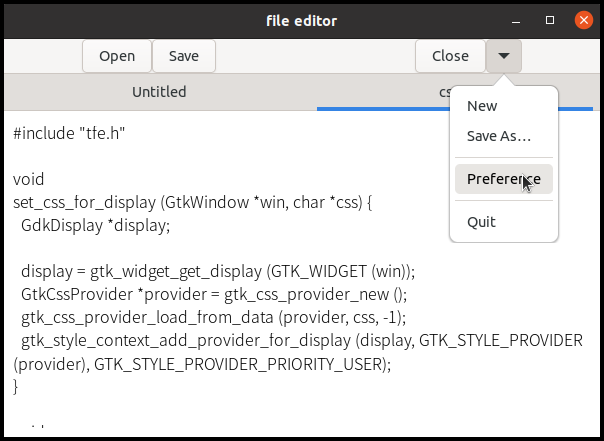
\includegraphics[width=9.06cm,height=6.615cm]{../image/tfe6.png}
\caption{tfe6}
\end{figure}

\begin{itemize}
\tightlist
\item
  Open, save and close buttons are placed on the toolbar. In addition,
  GtkMenuButton is added to the toolbar. This button shows a popup menu
  when clicked on. Here, popup means widely, including pull-down menu.
\item
  New, save-as, preference and quit items are put into the menu.
\end{itemize}

This makes the most frequently used operation bound to the tool bar
buttons. And the others are stored in behind the menus. So, it is more
practical.

The window is a composite widget. The definition is described in the XML
file \passthrough{\lstinline!tfewindow.ui!}.

\begin{lstlisting}[language=XML, numbers=left]
<?xml version="1.0" encoding="UTF-8"?>
<interface>
  <template class="TfeWindow" parent="GtkApplicationWindow">
    <property name="title">Text File Editor</property>
    <property name="default-width">600</property>
    <property name="default-height">400</property>
    <child>
      <object class="GtkBox" id="boxv">
        <property name="orientation">GTK_ORIENTATION_VERTICAL</property>
        <child>
          <object class="GtkBox" id="boxh">
            <property name="orientation">GTK_ORIENTATION_HORIZONTAL</property>
            <child>
              <object class="GtkLabel">
                <property name="width-chars">10</property>
              </object>
            </child>
            <child>
              <object class="GtkButton">
                <property name="label">Open</property>
                <property name="action-name">win.open</property>
              </object>
            </child>
            <child>
              <object class="GtkButton">
                <property name="label">Save</property>
                <property name="action-name">win.save</property>
              </object>
            </child>
            <child>
              <object class="GtkLabel">
                <property name="hexpand">TRUE</property>
              </object>
            </child>
            <child>
              <object class="GtkButton">
                <property name="label">Close</property>
                <property name="action-name">win.close</property>
              </object>
            </child>
            <child>
              <object class="GtkMenuButton" id="btnm">
                <property name="direction">down</property>
                <property name="icon-name">open-menu-symbolic</property>
              </object>
            </child>
            <child>
              <object class="GtkLabel">
                <property name="width-chars">10</property>
              </object>
            </child>
          </object>
        </child>
        <child>
          <object class="GtkNotebook" id="nb">
            <property name="scrollable">TRUE</property>
            <property name="hexpand">TRUE</property>
            <property name="vexpand">TRUE</property>
          </object>
        </child>
      </object>
    </child>
  </template>
</interface>
\end{lstlisting}

\begin{itemize}
\tightlist
\item
  Three buttons ``Open'', ``Save'' and ``Close'' are defined. You can
  use two ways to catch the button click event. The one is ``clicked''
  signal and the other is to register an action to the button. The first
  way is simple. You can connects the signal and your handler directly.
  The second way is like menu items. When the button is clicked, the
  corresponding action is activated. It is a bit complicated because you
  need to create an action and its ``activate'' handler in advance. But
  one advantage is you can connect two or more things to the action. For
  example, an accelerator can be connected to the action. Accelerators
  are keys that connects to actions. For example, Ctrl+O is often
  connected to a file open action. So, both open button and Ctrl+O
  activates an open action. The latter way is used in the XML file
  above.
\item
  You can specify a theme icon to GtkMenuButton with ``icon-name''
  poperty. The ``open-menu-symbolic'' is an image that is called
  hamburger menu.
\end{itemize}

The \passthrough{\lstinline!menu.ui!} XML file defines the menu for
GtkMenuButton.

\begin{lstlisting}[language=XML, numbers=left]
<?xml version="1.0" encoding="UTF-8"?>
<interface>
  <menu id="menu">
    <section>
      <item>
        <attribute name="label">New</attribute>
        <attribute name="action">win.new</attribute>
      </item>
      <item>
        <attribute name="label">Save As…</attribute>
        <attribute name="action">win.saveas</attribute>
      </item>
    </section>
    <section>
      <item>
        <attribute name="label">Preference</attribute>
        <attribute name="action">win.pref</attribute>
      </item>
    </section>
    <section>
      <item>
        <attribute name="label">Quit</attribute>
        <attribute name="action">win.close-all</attribute>
      </item>
    </section>
  </menu>
</interface>
\end{lstlisting}

There are four menu items and they are connected to actions.

\subsection{The header file}\label{the-header-file}

The following is the codes of \passthrough{\lstinline!tfewindow.h!}.

\begin{lstlisting}[language=C, numbers=left]
#pragma once

#include <gtk/gtk.h>

#define TFE_TYPE_WINDOW tfe_window_get_type ()
G_DECLARE_FINAL_TYPE (TfeWindow, tfe_window, TFE, WINDOW, GtkApplicationWindow)

void
tfe_window_notebook_page_new (TfeWindow *win);

void
tfe_window_notebook_page_new_with_files (TfeWindow *win, GFile **files, int n_files);

GtkWidget *
tfe_window_new (GtkApplication *app);
\end{lstlisting}

\begin{itemize}
\tightlist
\item
  5-6: \passthrough{\lstinline!TFE\_TYPE\_WINDOW!} definition and the
  \passthrough{\lstinline!G\_DECLARE\_FINAL\_TYPE!} macro.
\item
  8-15: Public functions. The first two functions creates a notebook
  page and the last function creates a window.
\end{itemize}

\subsection{C file}\label{c-file}

\subsubsection{A composite widget}\label{a-composite-widget}

The following codes are extracted from
\passthrough{\lstinline!tfewindow.c!}.

\begin{lstlisting}[language=C]
#include <gtk/gtk.h>
#include "tfewindow.h"

struct _TfeWindow {
  GtkApplicationWindow parent;
  GtkMenuButton *btnm;
  GtkNotebook *nb;
  gboolean is_quit;
};

G_DEFINE_FINAL_TYPE (TfeWindow, tfe_window, GTK_TYPE_APPLICATION_WINDOW);

static void
tfe_window_dispose (GObject *gobject) {
  gtk_widget_dispose_template (GTK_WIDGET (gobject), TFE_TYPE_WINDOW);
  G_OBJECT_CLASS (tfe_window_parent_class)->dispose (gobject);
}

static void
tfe_window_init (TfeWindow *win) {
  GtkBuilder *build;
  GMenuModel *menu;

  gtk_widget_init_template (GTK_WIDGET (win));

  build = gtk_builder_new_from_resource ("/com/github/ToshioCP/tfe/menu.ui");
  menu = G_MENU_MODEL (gtk_builder_get_object (build, "menu"));
  gtk_menu_button_set_menu_model (win->btnm, menu);
  g_object_unref(build);
... ... ...
}

static void
tfe_window_class_init (TfeWindowClass *class) {
  GObjectClass *object_class = G_OBJECT_CLASS (class);

  object_class->dispose = tfe_window_dispose;
  gtk_widget_class_set_template_from_resource (GTK_WIDGET_CLASS (class), "/com/github/ToshioCP/tfe/tfewindow.ui");
  gtk_widget_class_bind_template_child (GTK_WIDGET_CLASS (class), TfeWindow, btnm);
  gtk_widget_class_bind_template_child (GTK_WIDGET_CLASS (class), TfeWindow, nb);
}

GtkWidget *
tfe_window_new (GtkApplication *app) {
  return GTK_WIDGET (g_object_new (TFE_TYPE_WINDOW, "application", app, NULL));
}
\end{lstlisting}

The program above is similar to \passthrough{\lstinline!tfealert.c!} and
\passthrough{\lstinline!tfepref.c!}. It uses the same way to build a
composite widget. But there's one thing new. It is menu. The menu is
built from the XML resource \passthrough{\lstinline!menu.ui!} and
inserted into the menu button. It is done in the instance initialization
function \passthrough{\lstinline!tfe\_window\_init!}.

\subsubsection{Actions}\label{actions}

Actions can belong to an application or window. Tfe only has one top
window and all the actions are registered in the window. For example,
``close-all'' action destroys the top level window and that brings the
application to quit. You can make ``app.quit'' action instead of
``win.close-all''. It's your choice. If your application has two or more
windows, both ``app.quit'' and ``win:close-all'', which closes all the
notebook pages on the window, may be necessary. Anyway, you need to
consider that each action should belong to the application or a window.

Actions are defined in the instance initialization function.

\begin{lstlisting}[language=C]
static void
tfe_window_init (TfeWindow *win) {
... ... ...
/* ----- action ----- */
  const GActionEntry win_entries[] = {
    { "open", open_activated, NULL, NULL, NULL },
    { "save", save_activated, NULL, NULL, NULL },
    { "close", close_activated, NULL, NULL, NULL },
    { "new", new_activated, NULL, NULL, NULL },
    { "saveas", saveas_activated, NULL, NULL, NULL },
    { "pref", pref_activated, NULL, NULL, NULL },
    { "close-all", close_all_activated, NULL, NULL, NULL }
  };
  g_action_map_add_action_entries (G_ACTION_MAP (win), win_entries, G_N_ELEMENTS (win_entries), win);
... ... ...
}
\end{lstlisting}

Two things are necessary, an array and the
\passthrough{\lstinline!g\_action\_map\_add\_action\_entries!} function.

\begin{itemize}
\tightlist
\item
  The element of the array is the GActionEntry structure. The structure
  has the following members:

  \begin{itemize}
  \tightlist
  \item
    an action name
  \item
    a handler for the activate signal
  \item
    the type of the parameter or NULL for no parameter
  \item
    the initial state for the action
  \item
    a handler for the change-state signal
  \end{itemize}
\item
  The actions above are stateless and have no parameters. So, the third
  parameter and after are all NULL.
\item
  The function
  \passthrough{\lstinline!g\_action\_map\_add\_action\_entries!} adds
  the actions in the \passthrough{\lstinline!win\_entries!} array to the
  action map \passthrough{\lstinline!win!}. The last argument
  \passthrough{\lstinline!win!} is the user\_data, which is the last
  argument of handlers.
\item
  All the handlers are in \passthrough{\lstinline!tfewindow.c!} program
  and shown in the following subsections.
\end{itemize}

\subsubsection{The handlers of the
actions}\label{the-handlers-of-the-actions}

\paragraph{open\_activated}\label{open_activated}

The callback function \passthrough{\lstinline!open\_activated!} is an
activate signal handler on ``open'' action.

\begin{lstlisting}[language=C, numbers=left]
static void
open_activated (GSimpleAction *action, GVariant *parameter, gpointer user_data) {
  TfeWindow *win = TFE_WINDOW (user_data);
  GtkWidget *tv = tfe_text_view_new ();

  g_signal_connect (TFE_TEXT_VIEW (tv), "open-response", G_CALLBACK (open_response_cb), win);
  tfe_text_view_open (TFE_TEXT_VIEW (tv), GTK_WINDOW (win));
}
\end{lstlisting}

It connects the ``open-response'' signal on the newly created
TfeTextView instance and just calls
\passthrough{\lstinline!tfe\_text\_view\_open!}. It leaves the rest of
the task to the signal handler
\passthrough{\lstinline!open\_response\_cb!}.

\begin{lstlisting}[language=C, numbers=left]
static void
open_response_cb (TfeTextView *tv, int response, gpointer user_data) {
  TfeWindow *win = TFE_WINDOW (user_data);
  GFile *file;
  char *filename;

  if (response != TFE_OPEN_RESPONSE_SUCCESS) {
    g_object_ref_sink (tv);
    g_object_unref (tv);
  }else if (! G_IS_FILE (file = tfe_text_view_get_file (tv))) {
    g_object_ref_sink (tv);
    g_object_unref (tv);
  }else {
    filename = g_file_get_basename (file);
    g_object_unref (file);
    notebook_page_build (win, GTK_WIDGET (tv), filename);
    g_free (filename);
  }
}
\end{lstlisting}

If the TfeTextView instance failed to read a file, it destroys the
instance with \passthrough{\lstinline!g\_object\_ref\_sink!} and
\passthrough{\lstinline!g\_object\_unref!}. Since newly created widgets
are floating, you need to convert the floating reference to the normal
reference before you release it. The conversion is done with
\passthrough{\lstinline!g\_object\_ref\_sink!}.

If the instance successfully read the file, it calls
\passthrough{\lstinline!notebook\_page\_build!} to build a notebook page
and add it to the GtkNotebook object.

\begin{lstlisting}[language=C, numbers=left]
static void
notebook_page_build (TfeWindow *win, GtkWidget *tv, char *filename) {
  // The arguments win, tb and filename are owned by the caller.
  // If tv has a floating reference, it is consumed by the function.
  GtkWidget *scr = gtk_scrolled_window_new ();
  GtkTextBuffer *tb = gtk_text_view_get_buffer (GTK_TEXT_VIEW (tv));
  GtkNotebookPage *nbp;
  GtkWidget *lab;
  int i;

  gtk_text_view_set_wrap_mode (GTK_TEXT_VIEW (tv), GTK_WRAP_WORD_CHAR);
  gtk_scrolled_window_set_child (GTK_SCROLLED_WINDOW (scr), tv);
  lab = gtk_label_new (filename);
  i = gtk_notebook_append_page (win->nb, scr, lab);
  nbp = gtk_notebook_get_page (win->nb, scr);
  g_object_set (nbp, "tab-expand", TRUE, NULL);
  gtk_notebook_set_current_page (win->nb, i);
  g_signal_connect (GTK_TEXT_VIEW (tv), "change-file", G_CALLBACK (file_changed_cb), win->nb);
  g_signal_connect (tb, "modified-changed", G_CALLBACK (modified_changed_cb), tv);
}
\end{lstlisting}

This function is a kind of library function and it is called from the
different three places.

This function creates a new GtkScrolledWindow instance and sets its
child to \passthrough{\lstinline!tv!}. Then it appends it to the
GtkNotebook instance \passthrough{\lstinline!win->nb!}. And it sets the
tab label to the filename.

After the building, it connects two signals and handlers.

\begin{itemize}
\tightlist
\item
  ``change-file'' signal and \passthrough{\lstinline!file\_changed\_cb!}
  handler. If the TfeTextView instance changes the file, the handler is
  called and the notebook page tab is updated.
\item
  ``modified-changed'' signal and
  \passthrough{\lstinline!modified\_changed\_cb!} handler. If the text
  in the buffer of TfeTextView instance is modified, an asterisk is
  added at the beginning of the filename of the notebook page tab. If
  the text is saved to the file, the asterisk is removed. The asterisk
  tells the user that the text has been modified or not.
\end{itemize}

\begin{lstlisting}[language=C, numbers=left]
static void
file_changed_cb (TfeTextView *tv, gpointer user_data) {
  GtkNotebook *nb =  GTK_NOTEBOOK (user_data);
  GtkWidget *scr;
  GtkWidget *label;
  GFile *file;
  char *filename;

  file = tfe_text_view_get_file (tv);
  scr = gtk_widget_get_parent (GTK_WIDGET (tv));
  if (G_IS_FILE (file)) {
    filename = g_file_get_basename (file);
    g_object_unref (file);
  } else
    filename = get_untitled ();
  label = gtk_label_new (filename);
  g_free (filename);
  gtk_notebook_set_tab_label (GTK_NOTEBOOK (nb), scr, label);
}

static void
modified_changed_cb (GtkTextBuffer *tb, gpointer user_data) {
  TfeTextView *tv = TFE_TEXT_VIEW (user_data);
  GtkWidget *scr = gtk_widget_get_parent (GTK_WIDGET (tv));
  GtkWidget *nb =  gtk_widget_get_ancestor (GTK_WIDGET (tv), GTK_TYPE_NOTEBOOK);
  GtkWidget *label;
  GFile *file;
  char *filename;
  char *text;

  file = tfe_text_view_get_file (tv);
  filename = g_file_get_basename (file);
  if (gtk_text_buffer_get_modified (tb))
    text = g_strdup_printf ("*%s", filename);
  else
    text = g_strdup (filename);
  g_object_unref (file);
  g_free (filename);
  label = gtk_label_new (text);
  g_free (text);
  gtk_notebook_set_tab_label (GTK_NOTEBOOK (nb), scr, label);
}
\end{lstlisting}

\paragraph{save\_activated}\label{save_activated}

The callback function \passthrough{\lstinline!save\_activated!} is an
activate signal handler on ``save'' action.

\begin{lstlisting}[language=C, numbers=left]
static void
save_activated (GSimpleAction *action, GVariant *parameter, gpointer user_data) {
  TfeWindow *win = TFE_WINDOW (user_data);
  TfeTextView *tv = get_current_textview (win->nb);

  tfe_text_view_save (TFE_TEXT_VIEW (tv));
}
\end{lstlisting}

This function gets the current TfeTextView instance with the function
\passthrough{\lstinline!get\_current\_textview!}. And it just calls
\passthrough{\lstinline!tfe\_text\_view\_save!}.

\begin{lstlisting}[language=C, numbers=left]
static TfeTextView *
get_current_textview (GtkNotebook *nb) {
  int i;
  GtkWidget *scr;
  GtkWidget *tv;

  i = gtk_notebook_get_current_page (nb);
  scr = gtk_notebook_get_nth_page (nb, i);
  tv = gtk_scrolled_window_get_child (GTK_SCROLLED_WINDOW (scr));
  return TFE_TEXT_VIEW (tv);
}
\end{lstlisting}

\paragraph{close\_activated}\label{close_activated}

The callback function \passthrough{\lstinline!close\_activated!} is an
activate signal handler on ``close'' action. It closes the current
notebook page.

\begin{lstlisting}[language=C, numbers=left]
static void
close_activated (GSimpleAction *action, GVariant *parameter, gpointer user_data) {
  TfeWindow *win = TFE_WINDOW (user_data);
  TfeTextView *tv;
  GtkTextBuffer *tb;
  GtkWidget *alert;

  tv = get_current_textview (win->nb);
  tb = gtk_text_view_get_buffer (GTK_TEXT_VIEW (tv));
  if (! gtk_text_buffer_get_modified (tb)) /* is saved? */
    notebook_page_close (win);
  else {
    win->is_quit = FALSE;
    alert = tfe_alert_new_with_data ("Are you sure?", "Contents aren't saved yet.\nAre you sure to close?", "Close");
    gtk_window_set_transient_for (GTK_WINDOW (alert), GTK_WINDOW (win));
    g_signal_connect (TFE_ALERT (alert), "response", G_CALLBACK (alert_response_cb), win);
    gtk_window_present (GTK_WINDOW (alert));
  }
}
\end{lstlisting}

If the text in the current page has been saved, it calls
\passthrough{\lstinline!notebook\_page\_close!} to close the page.
Otherwise, it sets \passthrough{\lstinline!win->is\_quit!} to FALSE and
show the alert dialog. The ``response'' signal on the dialog is
connected to the handler \passthrough{\lstinline!alert\_response\_cb!}.

\begin{lstlisting}[language=C, numbers=left]
static void
notebook_page_close (TfeWindow *win){
  int i;

  if (gtk_notebook_get_n_pages (win->nb) == 1)
    gtk_window_destroy (GTK_WINDOW (win));
  else {
    i = gtk_notebook_get_current_page (win->nb);
    gtk_notebook_remove_page (win->nb, i);
  }
}
\end{lstlisting}

If the notebook has only one page, it destroys the window and the
application quits. Otherwise, it removes the current page.

\begin{lstlisting}[language=C, numbers=left]
static void
alert_response_cb (TfeAlert *alert, int response_id, gpointer user_data) {
  TfeWindow *win = TFE_WINDOW (user_data);

  if (response_id == TFE_ALERT_RESPONSE_ACCEPT) {
    if (win->is_quit)
      gtk_window_destroy(GTK_WINDOW (win));
    else
      notebook_page_close (win);
  }
}
\end{lstlisting}

If the user clicked on the cacel button, it does nothing. If the user
clicked on the accept button, which is the same as close button, it
calls \passthrough{\lstinline!notebook\_page\_close!}. Note that
\passthrough{\lstinline!win->is\_quit!} has been set to FALSE in the
\passthrough{\lstinline!close\_activated!} function.

\paragraph{new\_activated}\label{new_activated}

The callback function \passthrough{\lstinline!new\_activated!} is an
activate signal handler on ``new'' action.

\begin{lstlisting}[language=C, numbers=left]
static void
new_activated (GSimpleAction *action, GVariant *parameter, gpointer user_data) {
  TfeWindow *win = TFE_WINDOW (user_data);

  tfe_window_notebook_page_new (win);
}
\end{lstlisting}

It just calls
\passthrough{\lstinline!tfe\_window\_notebook\_page\_new!}, which is a
public method of TfeWindow.

\begin{lstlisting}[language=C, numbers=left]
void
tfe_window_notebook_page_new (TfeWindow *win) {
  GtkWidget *tv;
  char *filename;

  tv = tfe_text_view_new ();
  filename = get_untitled ();
  notebook_page_build (win, tv, filename);
  g_free (filename);
}
\end{lstlisting}

This function creates a new TfeTextView instance, ``Untitled'' family
string and calls \passthrough{\lstinline!notebook\_page\_build!}.

\paragraph{saveas\_activated}\label{saveas_activated}

The callback function \passthrough{\lstinline!saveas\_activated!} is an
activate signal handler on ``saveas'' action.

\begin{lstlisting}[language=C, numbers=left]
static void
saveas_activated (GSimpleAction *action, GVariant *parameter, gpointer user_data) {
  TfeWindow *win = TFE_WINDOW (user_data);
  TfeTextView *tv = get_current_textview (win->nb);

  tfe_text_view_saveas (TFE_TEXT_VIEW (tv));
}
\end{lstlisting}

This function gets the current page TfeTextView instance and calls
\passthrough{\lstinline!tfe\_text\_view\_saveas!}.

\paragraph{pref\_activated}\label{pref_activated}

The callback function \passthrough{\lstinline!pref\_activated!} is an
activate signal handler on ``pref'' action.

\begin{lstlisting}[language=C, numbers=left]
static void
pref_activated (GSimpleAction *action, GVariant *parameter, gpointer user_data) {
  TfeWindow *win = TFE_WINDOW (user_data);
  GtkWidget *pref;

  pref = tfe_pref_new ();
  gtk_window_set_transient_for (GTK_WINDOW (pref), GTK_WINDOW (win));
  gtk_window_present (GTK_WINDOW (pref));
}
\end{lstlisting}

This function creates a TfePref instance, which is a dialog, and sets
the transient parent window to \passthrough{\lstinline!win!}. And it
shows the dialog.

\paragraph{close\_all\_activated}\label{close_all_activated}

The callback function \passthrough{\lstinline!close\_all\_activated!} is
an activate signal handler on ``close\_all'' action.

\begin{lstlisting}[language=C, numbers=left]
static void
close_all_activated (GSimpleAction *action, GVariant *parameter, gpointer user_data) {
  TfeWindow *win = TFE_WINDOW (user_data);

  if (close_request_cb (win) == FALSE)
    gtk_window_destroy (GTK_WINDOW (win));
}
\end{lstlisting}

It first calls the function
\passthrough{\lstinline!close\_request\_cb!}. It is a callback function
for the ``close-request'' signal on the top window. It returns FALSE if
all the texts have been saved. Otherwise it returns TRUE.

Therefore, function \passthrough{\lstinline!close\_all\_activated!}
destroys the top window if all the texts have been saved. Otherwise it
does nothing. But, the function
\passthrough{\lstinline!close\_request\_cb!} shows an alert dialog and
if the user clicks on the accept button, the window will be destroyed.

\subsubsection{Window ``close-request''
signal}\label{window-close-request-signal}

GtkWindow has a ``close-request'' signal and it is emitted when the
close button, which is x-shaped button at the top right corner, is
clicked on. And the user handler is called before the default handler.
If the user handler returns TRUE, the rest of the close process is
skipped. If it returns FALSE, the rest will go on and the window will be
destroyed.

\begin{lstlisting}[language=C, numbers=left]
static gboolean
close_request_cb (TfeWindow *win) {
  TfeAlert *alert;

  if (is_saved_all (win->nb))
    return FALSE;
  else {
    win->is_quit = TRUE;
    alert = TFE_ALERT (tfe_alert_new_with_data ("Are you sure?", "Contents aren't saved yet.\nAre you sure to quit?", "Quit"));
    gtk_window_set_transient_for (GTK_WINDOW (alert), GTK_WINDOW (win));
    g_signal_connect (TFE_ALERT (alert), "response", G_CALLBACK (alert_response_cb), win);
    gtk_window_present (GTK_WINDOW (alert));
    return TRUE;
  }
}
\end{lstlisting}

First, it calls \passthrough{\lstinline!is\_saved\_all!} and checks if
the texts have been saved. If so, it returns FALSE and the close process
continues. Otherwise, it sets \passthrough{\lstinline!win->is\_quit!} to
TRUE and shows an alert dialog. When the user clicks on the accept or
cancel button, the dialog disappears and ``response'' signal is emitted.
Then, the handler \passthrough{\lstinline!alert\_response\_cb!} is
called. It destroys the top window if the user clicked on the accept
button since \passthrough{\lstinline!win->is\_quit!} is TRUE. Otherwise
it does nothing.

\begin{lstlisting}[language=C, numbers=left]
static gboolean
is_saved_all (GtkNotebook *nb) {
  int i, n;
  GtkWidget *scr;
  GtkWidget *tv;
  GtkTextBuffer *tb;

  n = gtk_notebook_get_n_pages (nb);
  for (i = 0; i < n; ++i) {
    scr = gtk_notebook_get_nth_page (nb, i);
    tv = gtk_scrolled_window_get_child (GTK_SCROLLED_WINDOW (scr));
    tb = gtk_text_view_get_buffer (GTK_TEXT_VIEW (tv));
    if (gtk_text_buffer_get_modified (tb))
      return FALSE;
  }
  return TRUE;
}
\end{lstlisting}

\subsubsection{Public functions}\label{public-functions}

There are three public functions.

\begin{itemize}
\tightlist
\item
  \passthrough{\lstinline!void tfe\_window\_notebook\_page\_new (TfeWindow *win)!}
\item
  \passthrough{\lstinline!void tfe\_window\_notebook\_page\_new\_with\_files (TfeWindow *win, GFile **files, int n\_files)!}
\item
  \passthrough{\lstinline!GtkWidget *tfe\_window\_new (GtkApplication *app)!}
\end{itemize}

The first function is called when the application emits the ``activate''
signal. The second is for ``open'' signal. It is given three arguments
and they are owned by the caller.

\begin{lstlisting}[language=C, numbers=left]
void
tfe_window_notebook_page_new_with_files (TfeWindow *win, GFile **files, int n_files) {
  int i;
  GtkWidget *tv;
  char *filename;

  for (i = 0; i < n_files; i++)
    if ((tv = tfe_text_view_new_with_file (*(files+i))) != NULL) {
      filename = g_file_get_basename (*(files+i));
      notebook_page_build (win, tv, filename);
      g_free (filename);
    }
  if (gtk_notebook_get_n_pages (win->nb) == 0)
    tfe_window_notebook_page_new (win);
}
\end{lstlisting}

This function has a loop for the array \passthrough{\lstinline!files!}.
It creates TfeTextView instance with the text from each file. And build
a page with it.

If an error happens and no page is created, it creates a new empty page.

\subsubsection{Full codes of
tfewindow.c}\label{full-codes-of-tfewindow.c}

The following is the full source codes of
\passthrough{\lstinline!tfewindow.c!}.

\begin{lstlisting}[language=C, numbers=left]
#include <gtk/gtk.h>
#include "tfewindow.h"
#include "tfepref.h"
#include "tfealert.h"
#include "../tfetextview/tfetextview.h"

struct _TfeWindow {
  GtkApplicationWindow parent;
  GtkMenuButton *btnm;
  GtkNotebook *nb;
  gboolean is_quit;
};

G_DEFINE_FINAL_TYPE (TfeWindow, tfe_window, GTK_TYPE_APPLICATION_WINDOW);

/* Low level functions */

/* Create a new untitled string */
/* The returned string should be freed with g_free() when no longer needed. */
static char*
get_untitled () {
  static int c = -1;
  if (++c == 0) 
    return g_strdup_printf("Untitled");
  else
    return g_strdup_printf ("Untitled%u", c);
}

/* The returned object is owned by the scrolled window. */
/* The caller won't get the ownership and mustn't release it. */
static TfeTextView *
get_current_textview (GtkNotebook *nb) {
  int i;
  GtkWidget *scr;
  GtkWidget *tv;

  i = gtk_notebook_get_current_page (nb);
  scr = gtk_notebook_get_nth_page (nb, i);
  tv = gtk_scrolled_window_get_child (GTK_SCROLLED_WINDOW (scr));
  return TFE_TEXT_VIEW (tv);
}

/* This call back is called when a TfeTextView instance emits a "change-file" signal. */
static void
file_changed_cb (TfeTextView *tv, gpointer user_data) {
  GtkNotebook *nb =  GTK_NOTEBOOK (user_data);
  GtkWidget *scr;
  GtkWidget *label;
  GFile *file;
  char *filename;

  file = tfe_text_view_get_file (tv);
  scr = gtk_widget_get_parent (GTK_WIDGET (tv));
  if (G_IS_FILE (file)) {
    filename = g_file_get_basename (file);
    g_object_unref (file);
  } else
    filename = get_untitled ();
  label = gtk_label_new (filename);
  g_free (filename);
  gtk_notebook_set_tab_label (GTK_NOTEBOOK (nb), scr, label);
}

static void
modified_changed_cb (GtkTextBuffer *tb, gpointer user_data) {
  TfeTextView *tv = TFE_TEXT_VIEW (user_data);
  GtkWidget *scr = gtk_widget_get_parent (GTK_WIDGET (tv));
  GtkWidget *nb =  gtk_widget_get_ancestor (GTK_WIDGET (tv), GTK_TYPE_NOTEBOOK);
  GtkWidget *label;
  GFile *file;
  char *filename;
  char *text;

  file = tfe_text_view_get_file (tv);
  filename = g_file_get_basename (file);
  if (gtk_text_buffer_get_modified (tb))
    text = g_strdup_printf ("*%s", filename);
  else
    text = g_strdup (filename);
  g_object_unref (file);
  g_free (filename);
  label = gtk_label_new (text);
  g_free (text);
  gtk_notebook_set_tab_label (GTK_NOTEBOOK (nb), scr, label);
}

static gboolean
is_saved_all (GtkNotebook *nb) {
  int i, n;
  GtkWidget *scr;
  GtkWidget *tv;
  GtkTextBuffer *tb;

  n = gtk_notebook_get_n_pages (nb);
  for (i = 0; i < n; ++i) {
    scr = gtk_notebook_get_nth_page (nb, i);
    tv = gtk_scrolled_window_get_child (GTK_SCROLLED_WINDOW (scr));
    tb = gtk_text_view_get_buffer (GTK_TEXT_VIEW (tv));
    if (gtk_text_buffer_get_modified (tb))
      return FALSE;
  }
  return TRUE;
}

static void
notebook_page_close (TfeWindow *win){
  int i;

  if (gtk_notebook_get_n_pages (win->nb) == 1)
    gtk_window_destroy (GTK_WINDOW (win));
  else {
    i = gtk_notebook_get_current_page (win->nb);
    gtk_notebook_remove_page (win->nb, i);
  }
}

static void
notebook_page_build (TfeWindow *win, GtkWidget *tv, char *filename) {
  // The arguments win, tb and filename are owned by the caller.
  // If tv has a floating reference, it is consumed by the function.
  GtkWidget *scr = gtk_scrolled_window_new ();
  GtkTextBuffer *tb = gtk_text_view_get_buffer (GTK_TEXT_VIEW (tv));
  GtkNotebookPage *nbp;
  GtkWidget *lab;
  int i;

  gtk_text_view_set_wrap_mode (GTK_TEXT_VIEW (tv), GTK_WRAP_WORD_CHAR);
  gtk_scrolled_window_set_child (GTK_SCROLLED_WINDOW (scr), tv);
  lab = gtk_label_new (filename);
  i = gtk_notebook_append_page (win->nb, scr, lab);
  nbp = gtk_notebook_get_page (win->nb, scr);
  g_object_set (nbp, "tab-expand", TRUE, NULL);
  gtk_notebook_set_current_page (win->nb, i);
  g_signal_connect (GTK_TEXT_VIEW (tv), "change-file", G_CALLBACK (file_changed_cb), win->nb);
  g_signal_connect (tb, "modified-changed", G_CALLBACK (modified_changed_cb), tv);
}

static void
open_response_cb (TfeTextView *tv, int response, gpointer user_data) {
  TfeWindow *win = TFE_WINDOW (user_data);
  GFile *file;
  char *filename;

  if (response != TFE_OPEN_RESPONSE_SUCCESS) {
    g_object_ref_sink (tv);
    g_object_unref (tv);
  }else if (! G_IS_FILE (file = tfe_text_view_get_file (tv))) {
    g_object_ref_sink (tv);
    g_object_unref (tv);
  }else {
    filename = g_file_get_basename (file);
    g_object_unref (file);
    notebook_page_build (win, GTK_WIDGET (tv), filename);
    g_free (filename);
  }
}

/* alert response signal handler */
static void
alert_response_cb (TfeAlert *alert, int response_id, gpointer user_data) {
  TfeWindow *win = TFE_WINDOW (user_data);

  if (response_id == TFE_ALERT_RESPONSE_ACCEPT) {
    if (win->is_quit)
      gtk_window_destroy(GTK_WINDOW (win));
    else
      notebook_page_close (win);
  }
}

/* ----- Close request on the top window ----- */
/* ----- The signal is emitted when the close button is clicked. ----- */
static gboolean
close_request_cb (TfeWindow *win) {
  TfeAlert *alert;

  if (is_saved_all (win->nb))
    return FALSE;
  else {
    win->is_quit = TRUE;
    alert = TFE_ALERT (tfe_alert_new_with_data ("Are you sure?", "Contents aren't saved yet.\nAre you sure to quit?", "Quit"));
    gtk_window_set_transient_for (GTK_WINDOW (alert), GTK_WINDOW (win));
    g_signal_connect (TFE_ALERT (alert), "response", G_CALLBACK (alert_response_cb), win);
    gtk_window_present (GTK_WINDOW (alert));
    return TRUE;
  }
}

/* ----- action activated handlers ----- */
static void
open_activated (GSimpleAction *action, GVariant *parameter, gpointer user_data) {
  TfeWindow *win = TFE_WINDOW (user_data);
  GtkWidget *tv = tfe_text_view_new ();

  g_signal_connect (TFE_TEXT_VIEW (tv), "open-response", G_CALLBACK (open_response_cb), win);
  tfe_text_view_open (TFE_TEXT_VIEW (tv), GTK_WINDOW (win));
}

static void
save_activated (GSimpleAction *action, GVariant *parameter, gpointer user_data) {
  TfeWindow *win = TFE_WINDOW (user_data);
  TfeTextView *tv = get_current_textview (win->nb);

  tfe_text_view_save (TFE_TEXT_VIEW (tv));
}

static void
close_activated (GSimpleAction *action, GVariant *parameter, gpointer user_data) {
  TfeWindow *win = TFE_WINDOW (user_data);
  TfeTextView *tv;
  GtkTextBuffer *tb;
  GtkWidget *alert;

  tv = get_current_textview (win->nb);
  tb = gtk_text_view_get_buffer (GTK_TEXT_VIEW (tv));
  if (! gtk_text_buffer_get_modified (tb)) /* is saved? */
    notebook_page_close (win);
  else {
    win->is_quit = FALSE;
    alert = tfe_alert_new_with_data ("Are you sure?", "Contents aren't saved yet.\nAre you sure to close?", "Close");
    gtk_window_set_transient_for (GTK_WINDOW (alert), GTK_WINDOW (win));
    g_signal_connect (TFE_ALERT (alert), "response", G_CALLBACK (alert_response_cb), win);
    gtk_window_present (GTK_WINDOW (alert));
  }
}

static void
new_activated (GSimpleAction *action, GVariant *parameter, gpointer user_data) {
  TfeWindow *win = TFE_WINDOW (user_data);

  tfe_window_notebook_page_new (win);
}

static void
saveas_activated (GSimpleAction *action, GVariant *parameter, gpointer user_data) {
  TfeWindow *win = TFE_WINDOW (user_data);
  TfeTextView *tv = get_current_textview (win->nb);

  tfe_text_view_saveas (TFE_TEXT_VIEW (tv));
}

static void
pref_activated (GSimpleAction *action, GVariant *parameter, gpointer user_data) {
  TfeWindow *win = TFE_WINDOW (user_data);
  GtkWidget *pref;

  pref = tfe_pref_new ();
  gtk_window_set_transient_for (GTK_WINDOW (pref), GTK_WINDOW (win));
  gtk_window_present (GTK_WINDOW (pref));
}

static void
close_all_activated (GSimpleAction *action, GVariant *parameter, gpointer user_data) {
  TfeWindow *win = TFE_WINDOW (user_data);

  if (close_request_cb (win) == FALSE)
    gtk_window_destroy (GTK_WINDOW (win));
}

/* --- public functions --- */

void
tfe_window_notebook_page_new (TfeWindow *win) {
  GtkWidget *tv;
  char *filename;

  tv = tfe_text_view_new ();
  filename = get_untitled ();
  notebook_page_build (win, tv, filename);
  g_free (filename);
}

void
tfe_window_notebook_page_new_with_files (TfeWindow *win, GFile **files, int n_files) {
  int i;
  GtkWidget *tv;
  char *filename;

  for (i = 0; i < n_files; i++)
    if ((tv = tfe_text_view_new_with_file (*(files+i))) != NULL) {
      filename = g_file_get_basename (*(files+i));
      notebook_page_build (win, tv, filename);
      g_free (filename);
    }
  if (gtk_notebook_get_n_pages (win->nb) == 0)
    tfe_window_notebook_page_new (win);
}

static void
tfe_window_dispose (GObject *gobject) {
  gtk_widget_dispose_template (GTK_WIDGET (gobject), TFE_TYPE_WINDOW);
  G_OBJECT_CLASS (tfe_window_parent_class)->dispose (gobject);
}

static void
tfe_window_init (TfeWindow *win) {
  GtkBuilder *build;
  GMenuModel *menu;

  gtk_widget_init_template (GTK_WIDGET (win));

  build = gtk_builder_new_from_resource ("/com/github/ToshioCP/tfe/menu.ui");
  menu = G_MENU_MODEL (gtk_builder_get_object (build, "menu"));
  gtk_menu_button_set_menu_model (win->btnm, menu);
  g_object_unref(build);

/* ----- action ----- */
  const GActionEntry win_entries[] = {
    { "open", open_activated, NULL, NULL, NULL },
    { "save", save_activated, NULL, NULL, NULL },
    { "close", close_activated, NULL, NULL, NULL },
    { "new", new_activated, NULL, NULL, NULL },
    { "saveas", saveas_activated, NULL, NULL, NULL },
    { "pref", pref_activated, NULL, NULL, NULL },
    { "close-all", close_all_activated, NULL, NULL, NULL }
  };
  g_action_map_add_action_entries (G_ACTION_MAP (win), win_entries, G_N_ELEMENTS (win_entries), win);

  g_signal_connect (GTK_WINDOW (win), "close-request", G_CALLBACK (close_request_cb), NULL);
}

static void
tfe_window_class_init (TfeWindowClass *class) {
  GObjectClass *object_class = G_OBJECT_CLASS (class);

  object_class->dispose = tfe_window_dispose;
  gtk_widget_class_set_template_from_resource (GTK_WIDGET_CLASS (class), "/com/github/ToshioCP/tfe/tfewindow.ui");
  gtk_widget_class_bind_template_child (GTK_WIDGET_CLASS (class), TfeWindow, btnm);
  gtk_widget_class_bind_template_child (GTK_WIDGET_CLASS (class), TfeWindow, nb);
}

GtkWidget *
tfe_window_new (GtkApplication *app) {
  return GTK_WIDGET (g_object_new (TFE_TYPE_WINDOW, "application", app, NULL));
}
\end{lstlisting}
